\documentclass[submit,techrep,noauthor]{ipsj}
\usepackage[dvipdfmx]{graphicx}
\usepackage{latexsym}
\usepackage{algorithm}
\usepackage{algorithmic}
\usepackage{amsmath}
\usepackage{url}

\begin{document}

\title{確信度ベース検証順序最適化による\\効率的コード生成候補選択}

\begin{abstract}
大規模言語モデル（LLM）によるコード生成では，複数候補を生成し，コンパイルとテストで採用候補を選ぶ運用が一般的である．本研究では，LLMが返すtoken-level log確率を用いた候補順位付けを評価し，log確率がコードの意味的正しさをどこまで予測できるかを調べる．候補全体の平均log確率で検証順序を決めるMean Log-Probability Ranking（Mean），局所的な低確率tokenを考慮するTail Log-Probability Ranking（Tail），極端な低確信度tokenを罰するExtreme-Mean（XMean）を比較する．主評価では，既存ベンチマーク，ParEval由来の問題，新規問題から20問を選抜し，同一プロンプトを独立に呼び出して得た$k=10$個の候補集合上でオフライン評価した．各手法は同一候補集合の検証順序のみを変えるため，成功率は生成順ベースラインGenと同じ78.2\%である．平均テスト数はGenの4.82回に対してMeanが4.48回，Tailが4.49回，XMeanが4.42回であった．20問を5問ずつ4ケースに分類すると，LogP-SeparableではXMeanが平均テスト数をGenの3.50回から2.52回へ削減した一方，LogP-Misleading / No-GainではGenより悪化した．これらの結果は，log確率は検証順序の軽量な手がかりにはなるが，意味的誤りの排除には不十分であり，極端な低確信度tokenを組み合わせても効果は問題依存であることを示す．
\end{abstract}

\maketitle


\section{はじめに}

LLMのコード生成能力は，Codex\cite{chen2021codex}やAlphaCode\cite{li2022alphacode}以降，大きく向上している．実用的なコード生成では，単一の出力をそのまま採用するのではなく，複数の候補を生成し，コンパイル，ユニットテスト，性能テストを通して採用候補を選択することが多い．この候補生成とテストに基づく選択は品質を高める一方で，候補数に比例して実行コストが増加する．

特にC言語性能最適化では，ループ展開，分岐削減，SIMD命令，キャッシュブロッキング，アルゴリズム変更など，多様な実装方針が存在する．LLMはこれらの候補を複数生成できるが，各候補の品質は一様ではない．生成順にテストするだけでは，成功候補が後方にある場合に余分なテストが必要となる．一方で，全候補をテストして最良候補を選択する方法は，成功率の観点では堅牢だが，テストコストが高い．

本研究の着眼点は，LLMが各トークンに対して出力するlog確率である．モデルが高い確率で生成したトークン列は，学習済みパターンと整合し，構文的に自然である可能性が高い．ただし，構文的な自然さは意味的正しさを保証しない．そこで，本研究では候補コード全体の平均log確率に基づくMeanと，局所的な低確率tokenを考慮するTailを比較し，token log確率が候補の正しさをどの程度識別できるかを評価する．

本研究の貢献は以下の3点である．
\begin{itemize}
\item \textbf{log確率ベース順位付けの限界分析}: 平均log確率を用いるMeanと局所tail確信度を用いるTailを比較し，高log確率でも意味的に誤る候補がMedium/Hardで多いことを示す．
\item \textbf{効果が出る問題特性の分析}: 20問をLogP-Separable，Extreme-Tail Sensitive，Sparse-Success / Limited Signal，LogP-Misleading / No-Gainの4ケースに分類し，log確率順位付けが有効になる条件を分析する．
\item \textbf{同一候補集合に基づく評価}: 候補生成の乱数差を排除するため，一度生成した候補集合を共有し，検証順序だけがテスト回数に与える影響をオフライン比較する評価手順を構築した．
\end{itemize}

以下，第2章で関連研究，第3章で予備知識，第4章で提案手法，第5章で実験設定，第6章で評価結果，第7章で考察，第8章で結論を述べる．

\section{関連研究}

\subsection{不確実性を用いたLLM出力制御}

Semantic Entropy\cite{semantic_entropy2024}は，意味的に同じ出力をクラスタリングし，意味空間でのエントロピーを計算することでLLMの幻覚検出精度を向上させた．
Code Semantic Entropy\cite{code_semantic_entropy2026}は，この考え方をコード生成に応用し，プログラムの振る舞いの多様性に基づいて問題レベルの不確実性を測定する．
Token-level不確実性に関しては，TokUR\cite{tokur2025}やtoken-level uncertainty-aware objective\cite{token_uq_training2025}が，低ランクランダム重み摂動やaleatoric/epistemic不確実性の分解により，トークン単位の信頼度評価や訓練目的への応用を検討している．

コード生成への不確実性の応用として，USCD（Uncertainty-Aware Selective Contrastive Decoding）\cite{uscd2024}は，token-level不確実性を用いて出力ノイズを除去し，negative promptとの対比的デコーディングを実施する手法を提案した．
また，Sharmaら\cite{assess_correctness2025}は，自然言語生成の不確実性推定技術をコード生成に適応し，symbolic executionで意味的等価性をクラスタリングすることで，LLM出力の正しさを不確実性で評価する手法を提案した．

本研究は，これらのtoken-level不確実性計測手法を候補選択の優先順位付けに適用する点で関連する．
USCDやsymbolic executionに基づく手法がデコーディング時介入や意味的等価性検証に焦点を当てるのに対し，本研究は生成後の候補検証順序の最適化を扱う．

\subsection{適応的デコーディング戦略}

AdaDec\cite{adadec2025}は，token-level不確実性（Shannon entropy）を用いたコード生成時の適応的デコーディング手法である．
高不確実性を検出したときにpause-then-rerank機構を実行し，lookaheadによりトークン選択を改善する．
AdaDecはデコーディング中のリアルタイム介入により単一候補の品質を向上させる手法である．

AdapT\cite{adapt2023}やEDT\cite{edt2024}は，トークンごとまたはステップごとに温度を適応的に調整する手法であり，生成品質と多様性のバランスを取る．
Semantic uncertainty in advanced decoding methods\cite{semantic_uncertainty_decoding2025}は，CoT等の高度なデコーディング手法におけるsemantic uncertaintyを調査し，デコーディング戦略が出力の多様性と信頼性に与える影響を分析した．
これらの手法がデコーディング時のパラメータ調整に焦点を当てるのに対し，本研究は生成済み候補の検証順序を最適化する．

\subsection{候補選択と反復的改善}

Self-Consistency\cite{wang2023selfconsistency}は，複数の推論経路をサンプリングし，最も一貫性のある解答を選択する手法で，コード生成でも複数候補選択の有効性を示唆する．
Codex\cite{chen2021codex}やAlphaCode\cite{li2022alphacode}は複数候補を生成し，テスト実行やクラスタリングで絞り込むが，候補の優先順位付けにLLMの確率情報を直接使用していない．
CodeT\cite{chen2022codet}は生成テストを用いて候補を評価し，CodeRL\cite{le2022coderl}はテスト結果を報酬として利用する．
本研究は，LLMの確信度（token-level確率の幾何平均）を用いた優先順位付けにより，生成済み候補のテスト回数削減を目指す．

反復的改善に関しては，Self-Refine\cite{madaan2023selfrefine}がLLM自身による反復的フィードバック・改善を提案したが，コード全体を対象とし，検証順序の最適化は扱わない．
UnCert-CoT\cite{uncert_cot2025}は不確実性定量化を取り入れ，挑戦的な側面を特定して選択的にCoT推論を活性化する．
AdaDecがデコーディング時のトークンレベル介入であるのに対し，本研究は生成後の候補選択と検証順序最適化を扱い，推論時に得られるtoken-level不確実性を利用する．

\subsection{確率較正とLLMの信頼性}

LLMの確率較正（calibration）は，出力確率が実際の正解率と一致するかを評価する．
Kadavathら\cite{kadavath2022language}は，言語モデルが自身の知識の境界を一定程度認識できることを示し，Xiongら\cite{xiong2023can}はLLMの不確実性表現能力を包括的に評価した．
SPUQ\cite{spuq2024}は入力摂動により不確実性を推定し，Expected Calibration Error（ECE）を平均50\%削減した．

コード生成タスクでの確率較正の検証はまだ限定的である．
本研究は，高確信候補が実際に高品質であるかを，候補検証順序と成功率・テスト回数の観点から評価する．
既存研究と比較した本研究の特徴は，(1) 生成後候補集合に対するテスト順序最適化，(2) 生成後検証における軽量な順位付け，(3) 既存の生成パイプラインに後処理として追加できる確信度利用，の3点である．

\section{予備知識}

\subsection{大規模言語モデルとコード生成}

大規模言語モデル（LLM）は，Transformerアーキテクチャを基盤とし，大規模なテキストコーパスとソースコードで事前学習された自己回帰型の生成モデルである．コード生成では，自然言語の問題記述，関数シグネチャ，制約条件，入出力例などを入力として，対応するプログラムをトークン列として生成する．

自己回帰生成では，モデルはそれまでに生成したトークン列$t_1,\ldots,t_{i-1}$に基づき，次トークン$t_i$の条件付き確率$P(t_i|t_1,\ldots,t_{i-1})$を計算する．生成時には，貪欲法，beam search，サンプリングなどにより次トークンが選択される．本研究では複数候補を得るため，温度付きサンプリングを用いる．

温度パラメータ$T$を用いたサンプリングでは，logit$s_i$から以下の分布を計算する．

\begin{equation}
P(t_i | t_1,\ldots,t_{i-1}) =
\frac{\exp(s_i/T)}{\sum_j \exp(s_j/T)}
\end{equation}

$T$が大きいほど分布は平坦になり，多様な候補が生成されやすい．一方，$T$が小さいほど高確率トークンに集中し，生成は決定的になる．本研究の主評価では，候補の多様性と品質のバランスを取るため，temperature=0.8を用いる．

\subsection{logprobsと確信度計算}

vLLM API\cite{kwon2023vllm}など，多くのLLM推論エンジンは，生成各トークンのlog確率（logprobs）を返す機能を提供する．logprobsは，そのトークンが選択される対数確率$\log P(t_i|t_1,\ldots,t_{i-1})$であり，モデルが各トークンをどの程度の確信を持って生成したかを表す．

本研究では，候補コード$c$の確信度を以下で定義する．

\begin{equation}
\text{conf}(c) = \exp\left(\frac{1}{N} \sum_{i=1}^{N} \log P(t_i)\right)
\end{equation}

ここで$N$は生成されたトークン数である．この値は，全トークン確率の幾何平均に相当する．単純な確率積を用いると長い候補ほど不利になるため，平均log確率を先に計算し，最後に指数化する．実装では，logprobが取得できない特殊トークンやNone値を除外して計算する．

確信度が候補品質の指標となり得る理由は，以下の4点である．

\begin{itemize}
\item \textbf{学習データとの類似性}: 高確信度は，モデルが学習データ中で頻繁に観測したコードパターンと整合していることを示す．ループ展開や分岐削減のような定型的な最適化は，高確信度で生成されやすい．
\item \textbf{構文的一貫性}: 各トークンが高確率で選択されるコードは，局所的な構文や識別子の使い方が一貫している可能性が高い．低確信度トークンが多い場合，構文エラーや関数シグネチャの不一致が生じやすい．
\item \textbf{実装方針の安定性}: モデルが複数の実装方針の間で迷う場合，トークン確率は分散し，確信度が低下する．アルゴリズム変更やデータ構造実装では，境界条件，再帰終了条件，メモリ管理などでこの傾向が現れる．
\item \textbf{経験的相関}: Kadavathら\cite{kadavath2022language}は，LLMの確率出力と正解率に相関があることを示した．本研究の評価においても，成功候補は高確信度側に多く，失敗候補は低確信度側に多い傾向が確認された（詳細は第6章）．
\end{itemize}

\subsection{vLLM API}

vLLM\cite{kwon2023vllm}は，PagedAttentionを用いた高速なLLM推論エンジンであり，OpenAI互換APIとして利用できる．本研究では，Qwen3.5-9B-AWQ-4bitをvLLM経由で利用した．vLLM APIでは，\texttt{logprobs}パラメータを指定することで，生成トークンとともに上位候補トークンのlog確率を取得できる．

本手法の実装では，各候補について生成テキストとtoken-level logprobsを同時に取得する．その後，コードブロックを抽出し，候補単位の確信度を計算する．この処理は生成後に行うため，デコーディングアルゴリズム自体を変更する必要がない．したがって，log確率に基づく検証順序最適化は既存のvLLMベースのコード生成パイプラインに後処理として追加できる．

\subsection{性能最適化タスク}

本研究の評価対象は，C言語の性能最適化タスクである．各問題では，指定された関数シグネチャに従って関数を実装し，コンパイルとテストに通過することを成功条件とする．問題には，配列和や疎行列ベクトル積のループ最適化，分岐削減，SIMD風のベクトル演算，混合精度計算，ソートやグラフ計算などが含まれる．ループ展開は複数回の反復をまとめてループ制御オーバーヘッドを削減するが，剰余要素の処理を誤ると正しさを損なう．分岐削減は条件分岐を算術演算等に置き換えるが，境界条件の実装を誤ると結果が変わる．アルゴリズム変更は計算量の異なる実装へ置き換えるが，関数全体の構造，補助関数，再帰，境界条件を正しく実装する必要があり，LLMにとって難度が高い．また，ステンシル計算や混合精度正規化のように，構文的には自然でも数値誤差や境界条件で失敗しやすい問題も含まれる．


\section{提案手法}


\subsection{log確率に基づく検証順序最適化}

本稿では，LLMが出力するtoken-level log確率から候補コードの確信度を計算し，その確信度に基づいて検証順序を制御する．扱う選択規則は，平均log確率を用いるMean Log-Probability Ranking（Mean），局所的な低確率tokenを考慮するTail Log-Probability Ranking（Tail），極端な低確信度tokenを罰するExtreme-Mean（XMean）である．

\begin{itemize}
\item \textbf{Mean}: 固定候補数$k$個の候補を生成し，平均log確率に基づく確信度順に検証する．
\item \textbf{Tail}: 固定候補数$k$個の候補を生成し，token log確率の下位四分位に基づいて検証する．
\item \textbf{XMean}: 固定候補数$k$個の候補を生成し，平均log確率から極端な低確信度tokenの割合を罰則として差し引いたスコアで検証する．
\end{itemize}

Mean，Tail，XMeanはいずれも同じ固定候補集合に対する検証順序制御であり，候補集合そのものはGenと共有する．そのため，候補集合中に成功候補が存在するかどうかは全手法で同じであり，成功率は検証順序に依存しない．本稿の主目的は，成功率ではなく，成功候補に到達するまでのテスト回数を削減できるかを評価することである．

\subsection{Mean，Tail，XMean}

Meanは，固定候補数$k$個の候補を生成し，平均log確率に基づく確信度順に検証することで，成功候補に到達するまでの平均テスト数を削減する手法である．同一候補集合を用いるため成功率はベースライン（全候補を検証）と同等だが，検証順序を最適化することで無駄なテストを削減できる．

Algorithm~\ref{alg:mean_logp}にMeanを示す．まずLLMから$k$個の候補を生成し，各候補のlogprobsから平均log確率に基づく確信度を計算する．次に候補を確信度の降順に並べ替え，順にコンパイル・テストする．成功候補が見つかれば，その時点で終了し，残りの候補の検証を省略する．全候補が失敗した場合は失敗として扱う．

この手法は，候補プール内の成功候補が高確信度側に偏っている場合に有効である．例えば，$k=10$の候補のうち確信度1位が成功候補であれば，テスト数は1回で済む．一方，成功候補が確信度10位であれば，テスト数は10回となる．したがって，平均テスト数は成功候補の確信度順位に依存する．

平均log確率は候補全体の自然さを表す一方で，局所的に極端に低確率なtokenの存在を十分に反映しない場合がある．そこで本稿では，固定候補集合の別の順位付け規則としてTailを定義する．Tailでは，候補$c$のtoken log確率列$\{\ell_i\}_{i=1}^{N}$に対し，下位四分位
\begin{equation}
\text{tail}(c) = Q_{0.25}(\{\ell_i\}_{i=1}^{N})
\end{equation}
を局所tail確信度として用い，$\text{tail}(c)$の降順に候補を検証する．これは，平均的には自然でも一部に低確率tokenを含む候補を後回しにすることを意図した規則である．

さらに，全token分布の分析から，失敗候補では下位四分位よりもさらに右端の極端な低確信度tokenが有効な手がかりになる場合があることが分かった．そこでXMeanでは，loss $-\ell_i$が6以上となるtokenの割合
\begin{equation}
r_6(c) = \frac{1}{N}\left|\{i \mid -\ell_i \geq 6\}\right|
\end{equation}
を用い，
\begin{equation}
\text{xmean}(c) = \frac{1}{N}\sum_{i=1}^{N}\ell_i - 100r_6(c)
\end{equation}
の降順に候補を検証する．これは，平均的には高確信度でも局所的に極端に怪しいtokenを含む候補を後回しにすることを意図した規則である．

\begin{algorithm}[t]
\caption{Mean Log-Probability Ranking}
\label{alg:mean_logp}
\begin{algorithmic}[1]
\REQUIRE 問題記述$P$，候補数$k$
\ENSURE 成功したコード候補または失敗
\STATE 候補集合$C=\{c_1,\ldots,c_k\}$をLLMで生成し，logprobsを取得
\FOR{各候補$c_j \in C$}
    \STATE $\text{conf}(c_j)=\exp(\frac{1}{N_j}\sum_i \log P(t_i))$を計算
\ENDFOR
\STATE $C$を$\text{conf}(c_j)$の降順に整列
\FOR{各候補$c_j \in C$}
    \STATE $c_j$をコンパイルし，テストを実行
    \IF{$c_j$が成功}
        \RETURN $c_j$
    \ENDIF
\ENDFOR
\RETURN 失敗
\end{algorithmic}
\end{algorithm}

\section{実験設定}

\subsection{環境}

実験では，Qwen3.5-9B-AWQ-4bitをvLLM\cite{kwon2023vllm}経由で利用し，OpenAI互換APIからlogprobsを取得した．生成パラメータはtemperature=0.8，候補数は全評価で$k=10$に統一した．推論にはchat completion APIを用い，thinking出力はchat templateの設定で無効化した．max\_tokensは4096とした．生成されたCコードはgcc 14.3.1で\texttt{-O3 -lm}を付けてコンパイルし，各問題に付属するテストプログラムを実行した．実験環境はLinux 6.12，Python 3.12.12，Intel Xeon Platinum 8368 CPUである．主評価では20問それぞれについて50試行を行い，合計1000試行を評価した．コード生成時の乱数seedはvLLM API側で固定していないため，完全な再生成再現性は保証しない．一方，主評価では全候補のコード，確信度，コンパイル・テスト結果，エラー種別をJSONに保存し，解析の再現性を確保した．


\subsection{比較手法}

ここで，主評価における候補の生成方法を明示する．各問題には，5.4節で述べる通常の最適化指示プロンプト$P$がある．これは問題の目的，関数シグネチャ，実装上の制約，``Return only C code.''，``Required \#include directives and helper definitions are allowed.''，``Do not include markdown fences or explanatory text.'' という最小限の出力制約を含む基本プロンプトである．主評価では，プロンプト内で複数解の列挙を要求するのではなく，各問題・各試行について同じプロンプト$P$を$k=10$回独立にAPIへ送信し，1回の呼び出しから1個の候補を得る．これにより候補集合$C=\{c_0,\ldots,c_{k-1}\}$を構成する．

本稿の比較手法はすべて，この同一候補プールに対する\textbf{選択規則}の違いとして定義する．実運用時の各手法は成功候補が見つかった時点で停止するが，実験では候補集合を固定して比較するため，まず全候補をコンパイル・テストして候補単位の成否とlog確率統計を保存し，その後に各規則をオフライン評価する．

\begin{itemize}
\item \textbf{Gen}: 同一プロンプトから得た共有候補プールをAPIの返却順$c_0,\ldots,c_{k-1}$にテストし，最初に成功した候補を採用する生成順早期停止である．
\item \textbf{Mean}: 共有候補プール全体を使い，平均log確率に基づく確信度の降順に候補をテストするMean Log-Probability Rankingである．
\item \textbf{Tail}: 共有候補プール全体を使い，token log確率の下位四分位$\text{tail}(c)$の降順に候補をテストするTail Log-Probability Rankingである．
\item \textbf{XMean}: Meanに極端な低確信度tokenの割合を罰則として加えるExtreme-Meanである．候補$c$の平均log確率を$\overline{\ell}(c)$，$-\ell_i \geq 6$となるtoken割合を$r_6(c)$とし，$\overline{\ell}(c)-100r_6(c)$の降順に候補をテストする．
\end{itemize}

この設計により，候補集合の違いによる成功率の揺らぎを排除し，検証順序だけがテスト数と採用候補に与える影響を評価できる．Gen，Mean，Tail，XMeanはいずれも同じ候補集合を成功候補が見つかるまで，または全候補が失敗するまで検証する．したがって，各試行の成功条件は「候補集合中に少なくとも1個の成功候補が存在すること」であり，成功率は手法間で同一である．

\subsection{ベンチマーク}

本研究では，既存ベンチマーク，ParEval由来の問題，新規に作成した数値・検証問題から20問を選抜した．本稿では，コードの題材だけでなく，log確率に基づく順位付けがどのように効いたかを分析するため，20問を5問ずつ4ケースに分類する．これは事前難易度ではなく，候補集合上で観察された確信度信号の振る舞いに基づく分析用分類である．

\begin{itemize}
\item \textbf{LogP-Separable}: MeanまたはTailだけでGenより明確に少ないテスト数を達成した問題群である．成功候補と失敗候補のlog確率統計が比較的分離する．
\item \textbf{Extreme-Tail Sensitive}: 下位四分位だけでは十分でないが，極端に低確信度なtokenを罰するXMeanが改善しやすい問題群である．
\item \textbf{Sparse-Success / Limited Signal}: 候補集合内の成功候補が少ない，または成功候補があってもlog確率信号が弱く，改善余地が限定される問題群である．
\item \textbf{LogP-Misleading / No-Gain}: log確率に基づく順位付けがほぼ効かない，またはGenより悪化する問題群である．意味的誤りが自然なtoken列として生成される場合を含む．
\end{itemize}

この構成により，単に成功率の高低で分けるのではなく，Mean，Tail，XMeanがどのような候補集合で有効になるかを分析できる．表\ref{tab:task_details}に各ベンチマークの詳細を示す．

\subsection{プロンプト設計}

本研究でLLMに生成させるコードは，完全なプログラムではなく，指定されたC関数または関連する関数群の実装である．各問題にはテスト用の\texttt{main}関数を含むテストプログラムが付属しており，LLMの出力コードをテストプログラムとリンクしてコンパイル・実行する．したがって，生成候補は関数シグネチャを満たし，テストプログラムが期待する副作用や戻り値を実装する必要がある．

\begin{table*}[t]
\caption{生成対象となるCコードの内容（20課題）}
\label{tab:task_details}
\centering
\scriptsize
\setlength{\tabcolsep}{3pt}
\begin{tabular*}{\textwidth}{@{\extracolsep{\fill}}p{0.16\textwidth}p{0.20\textwidth}p{0.14\textwidth}p{0.44\textwidth}@{}}
\hline
ベンチマーク & 集合 & カテゴリ & 生成対象コード \\
\hline
Sort Nonzero & LogP-Separable & Sorting & ゼロ位置を固定したまま，非ゼロ要素のみを昇順に並べ替える． \\
UTF-8 Validate & LogP-Separable & Validation & UTF-8列について過長符号化，surrogate，範囲外code pointを厳密に拒否する． \\
Largest Component & LogP-Separable & Graph & グリッドまたはグラフ上の連結成分を探索し，最大成分サイズを返す． \\
Crop2D & LogP-Separable & Stride & 入力strideと出力paddingを持つ2次元cropを実装し，padding領域を変更しない． \\
SpMV & LogP-Separable & Sparse & CSR形式の疎行列ベクトル積，AXPY，内積を一回の走査で融合する． \\
\hline
Conv2D & Extreme-Tail & Convolution & NHWC配置のmulti-channel 3x3 valid convolutionを実装する． \\
Transpose & Extreme-Tail & Cache & 行列転置をブロック単位に分割してキャッシュ局所性を高める． \\
Radix & Extreme-Tail & Sorting & キーと値の対応を保持する安定radix sortを実装する． \\
RMSNorm & Extreme-Tail & Reduction & RMSNormの二乗和計算をdoubleで蓄積して丸め誤差を抑える． \\
HeapSort & Extreme-Tail & Heap & ヒープ構造の構築・維持とソート処理を正しく実装する． \\
\hline
Banded Edit & Sparse/Limited & Dynamic Prog. & 帯幅制約付き編集距離を計算し，帯外遷移を扱う． \\
Convex Hull & Sparse/Limited & Geometry & 重複点や共線点を含む点集合に対して凸包周長を計算する． \\
Top-k NaN & Sparse/Limited & Selection & NaNを無視して浮動小数点配列の上位k要素を選択する． \\
Stencil3D & Sparse/Limited & Stencil & 3次元7点ステンシルを境界条件と精度制約を満たして実装する． \\
Stencil2D & Sparse/Limited & Stencil & halo領域を含む2次元ステンシル計算を実装する． \\
\hline
Floyd & Misleading/No-Gain & Graph & 全点対最短路をFloyd-Warshallアルゴリズムでin-place更新する． \\
Strided Transpose & Misleading/No-Gain & Stride & 入出力strideを持つ矩形行列転置を実装し，出力paddingを保持する． \\
Triangular Solve & Misleading/No-Gain & Solver & 複数右辺の下三角ソルバをstride付き行列上で実装する． \\
Quadratic Roots & Misleading/No-Gain & Numerics & 桁落ちを避ける二次方程式の安定な解法を実装する． \\
Cholesky SPD & Misleading/No-Gain & Linear Algebra & 対称正定値行列のCholesky分解を行い，非正定値入力を検出する． \\
\hline
\end{tabular*}
\end{table*}

生成プロンプトは，各問題の目的，関数シグネチャ，実装上の指示，出力制約からなる．典型的には，``Implement an optimized ... in C''で最適化対象を指定し，``Function signature:''または``Function signatures:''で必要な関数を列挙する．続いて，ループ展開，分岐削減，キャッシュ局所性，配列ベースデータ構造，数値安定化など，期待する実装方針を自然言語で与える．最後に，Cコードのみを出力し，必要な\texttt{\#include}と補助定義は許可し，Markdownフェンスや説明文を含めないという最小限の制約を付ける．

例えば，Strided Transposeでは，入力要素\texttt{in[i*in\_stride+j]}を出力要素\texttt{out[j*out\_stride+i]}へ書き込み，padding領域を変更しないよう指示する．Radixでは，キーと値の対応を保持した安定ソートを実装するよう指示する．Sort Nonzeroでは，ゼロ値の位置を保持しながら非ゼロ要素のみを整列する制約を明示する．RMSNormでは，float入出力に対してdouble蓄積を用い，テストで要求される誤差閾値を満たすよう指示する．UTF-8検証では，過長符号化やsurrogateを拒否する境界条件を明示し，Cholesky分解では非正定値入力を検出して失敗を返すよう指示する．Convex Hullでは重複点や共線点の扱いを明示する．このように，プロンプトは単なる関数名だけでなく，期待する最適化方針と正しさに必要な条件を含む．主評価の共有候補プールでは，同一の問題プロンプトを独立に10回呼び出して候補を生成し，候補間の改善指示は用いない．したがって，主評価の候補集合は段階的な改善系列ではなく，同一プロンプト条件下で得た10候補である．

\subsection{評価指標}

成功率は，コンパイルに成功し，テストプログラムがPASSを出力した候補を採用できた試行の割合である．本稿の比較手法は同一候補集合の順序だけを変えるため，成功率は手法別の性能差ではなく，候補集合自体の品質を表す補助指標である．平均テスト数は，各選択規則が成功または全失敗を確定するまでに必要とする候補テスト数を，問題数と試行数で割った値である．全候補検証では常に$k$となり，早期停止方式では成功候補の順位に応じて小さくなる．

MeanおよびTailは生成済み候補の検証順序を決める手法であり，候補集合内に成功候補が存在しない試行を成功させることはできない．そこで，候補生成品質を表す指標として，全候補を検証したときに少なくとも1個の成功候補が存在した試行数も確認する．

\section{評価}


\subsection{主要評価}

各手法を同一候補プール上で評価する．図中では，生成順ベースラインをGen，平均log確率順位をMean，局所tail順位をTail，極端な低確信度tokenを罰する順位をXMeanと略記する．4ケースの評価結果を図\ref{fig:case_logp_separable}--\ref{fig:case_logp_misleading}に示す．上段の確信度分布では破線が confidence=0.75 を示し，タイトル下の括弧内にその閾値以上での成功率を示す．また，高確信度領域にある失敗候補を赤いrugマークで示す．下段はtrial単位のテスト数の箱ひげ図である．箱は四分位範囲，中央線は中央値，ヒゲは1.5 IQR内の範囲，色付きひし形は平均値を示す．

\begin{figure*}[t]
\centering
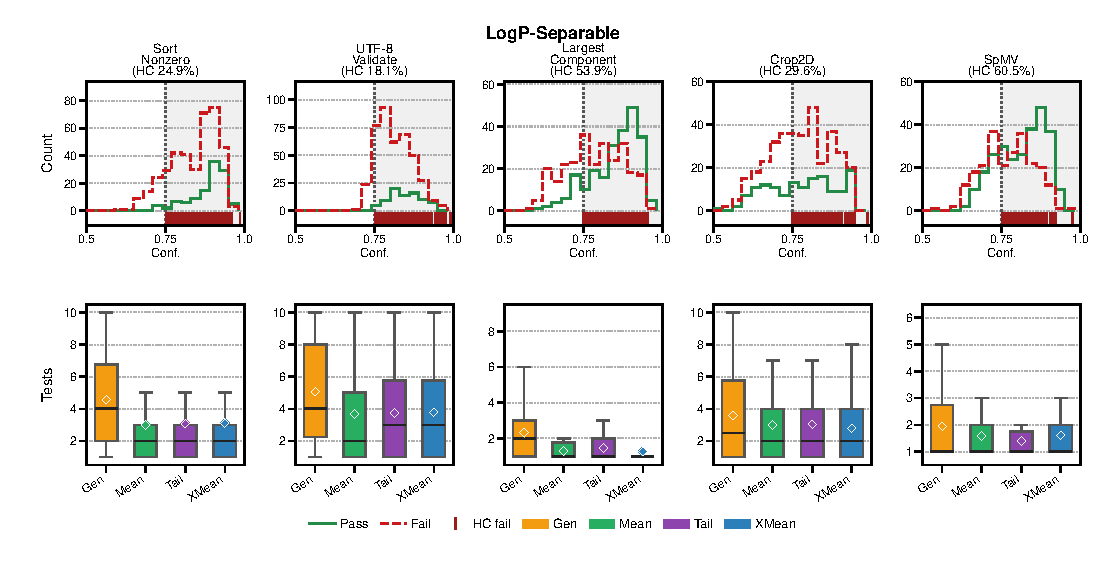
\includegraphics[width=\textwidth]{cbba_case_logp_separable.eps}
\caption{LogP-Separableケース（Sort Nonzero, UTF-8 Validate, Largest Component, Crop2D, SpMV）の評価結果．成功候補と失敗候補のlog確率統計が比較的分離し，Mean，Tail，XMeanがGenより大きくテスト数を削減した．}
\label{fig:case_logp_separable}
\end{figure*}

\begin{figure*}[t]
\centering
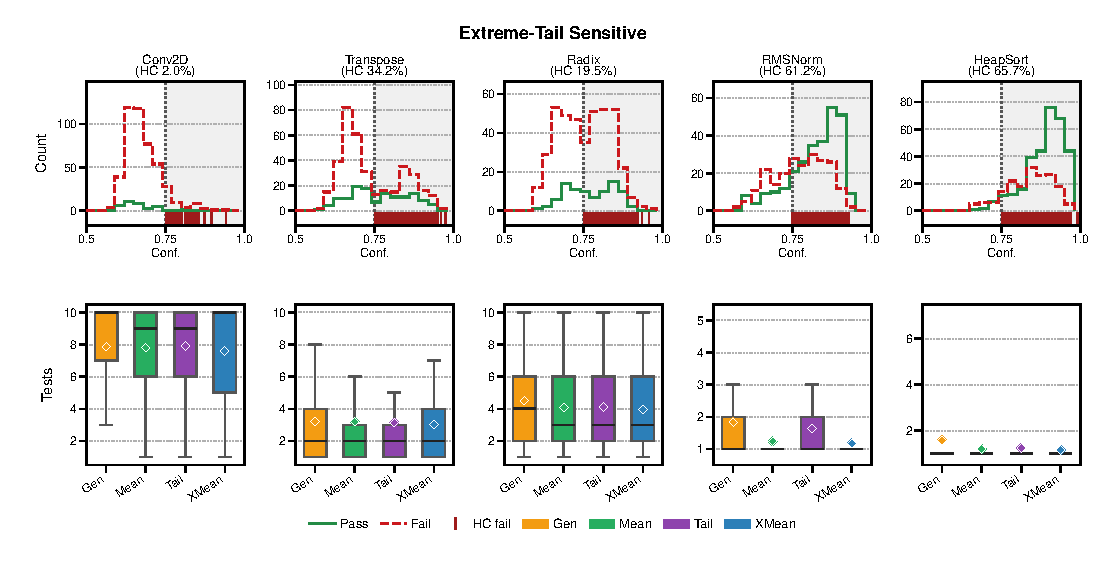
\includegraphics[width=\textwidth]{cbba_case_extreme_tail_sensitive.eps}
\caption{Extreme-Tail Sensitiveケース（Conv2D, Transpose, Radix, RMSNorm, HeapSort）の評価結果．下位四分位だけでは十分でないが，極端に低確信度なtokenを罰するXMeanが改善しやすい問題群である．}
\label{fig:case_extreme_tail}
\end{figure*}

\begin{figure*}[t]
\centering
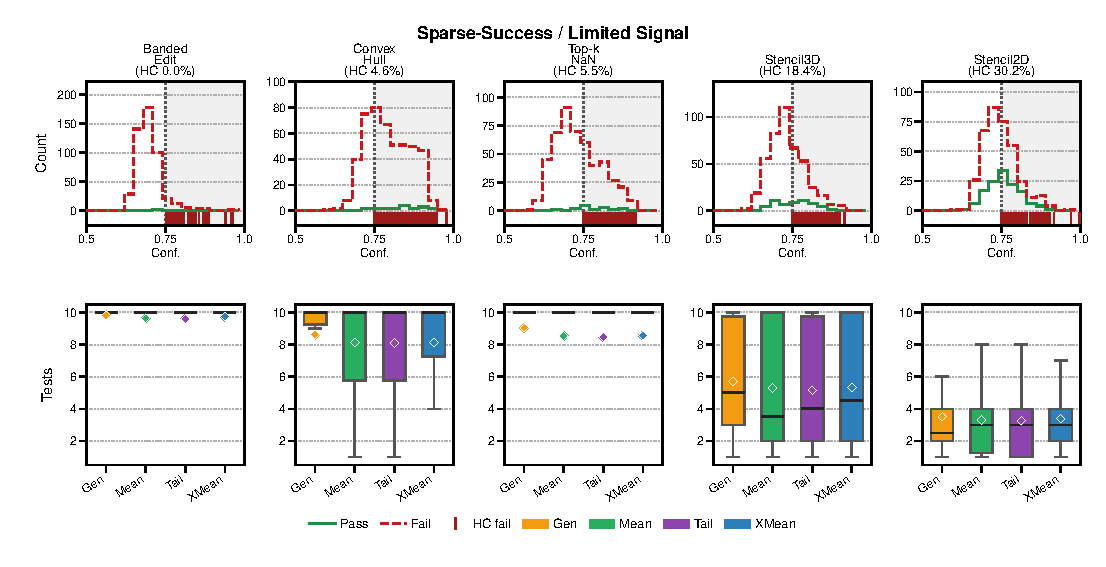
\includegraphics[width=\textwidth]{cbba_case_sparse_success_limited_signal.eps}
\caption{Sparse-Success / Limited Signalケース（Banded Edit, Convex Hull, Top-k NaN, Stencil3D, Stencil2D）の評価結果．候補集合内の成功候補が少ない，またはlog確率信号が弱く，改善後もテスト数が高めに残る．}
\label{fig:case_sparse_signal}
\end{figure*}

\begin{figure*}[t]
\centering
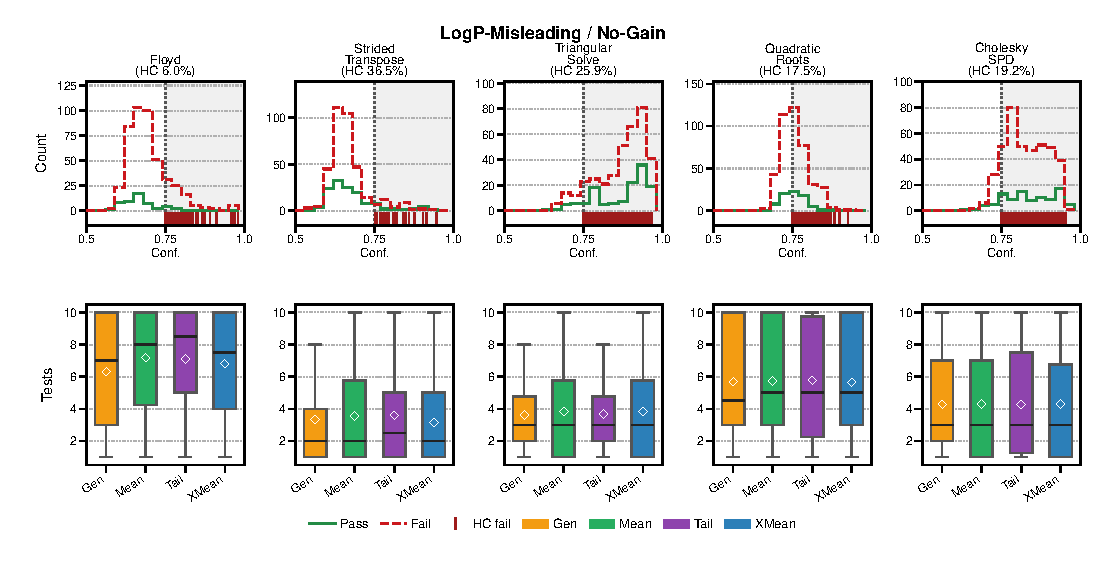
\includegraphics[width=\textwidth]{cbba_case_logp_misleading_no_gain.eps}
\caption{LogP-Misleading / No-Gainケース（Floyd, Strided Transpose, Triangular Solve, Quadratic Roots, Cholesky SPD）の評価結果．log確率に基づく順位付けがほぼ効かない，またはGenより悪化する問題群である．}
\label{fig:case_logp_misleading}
\end{figure*}

\begin{figure*}[t]
\centering
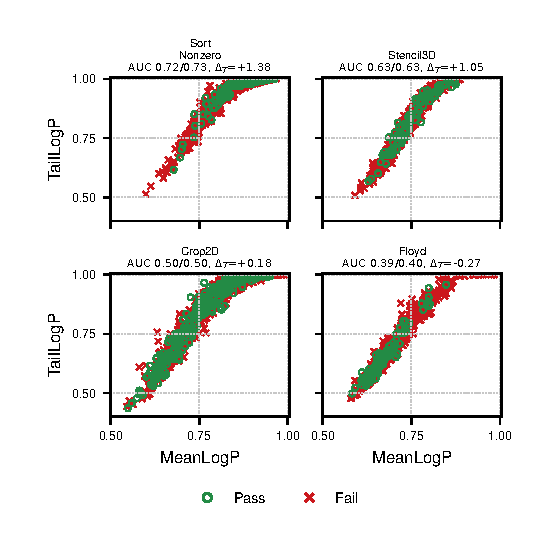
\includegraphics[width=\textwidth]{token_logp_feature_space.eps}
\caption{各候補のMeanLogPとTailLogPの分布．9Bモデル，$k=10$で評価した20ベンチマークについて，各点は1候補を表し，横軸は平均token log確率に基づく確信度，縦軸はtoken log確率の下位四分位に基づくtail確信度である．緑はテスト成功候補，赤は失敗候補を示す．各パネルのAUCは，成功候補を失敗候補より高く順位付けできる確率をMean/Tailの順に示し，$\Delta_T$はGenに対するTailの平均テスト数削減量を表す．各パネルは$\Delta_T$の降順に並べた．}
\label{fig:token_logp_feature_space}
\end{figure*}

\begin{figure*}[t]
\centering
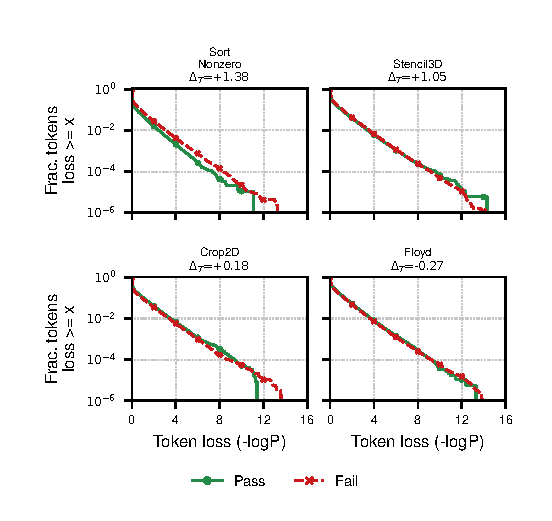
\includegraphics[width=\textwidth]{token_loss_distribution.eps}
\caption{全tokenの低確信度側分布．9Bモデル，$k=10$で評価した20ベンチマークについて，成功候補に含まれるtokenと失敗候補に含まれるtokenを集約し，token loss $-\log P(t)$ の生存分布を示す．縦軸はlossが横軸値以上となるtokenの割合であり，右側の裾が長いほど低確信度tokenを多く含む．各パネルはTailによる平均テスト数削減量$\Delta_T$の降順に並べた．全tokenを点で描くと過密になるため，約1680万tokenを分布として集約した．}
\label{fig:token_loss_distribution}
\end{figure*}

図\ref{fig:token_logp_feature_space}は，MeanとTailが実際に参照する2つのlog確率統計量を候補単位で可視化したものである．成功候補と失敗候補が右上方向で分離している問題では，log確率に基づく順位付けが有効に働く．一方，成功候補と失敗候補が大きく重なる問題では，高確信度でも意味的に誤る候補が多く，log確率だけでは検証前に失敗を十分に排除できない．TailがMeanより高いAUCを示す問題では，候補全体の平均的な自然さよりも，局所的な低確率tokenの少なさが成功候補の順位付けに有効であることを示している．
図\ref{fig:token_loss_distribution}は，同じ現象をtoken単位で見たものである．失敗候補の曲線が成功候補より上側にある領域では，失敗候補が低確信度tokenを多く含んでいることを意味する．今回の20問分析では，loss $\ge 4$となる低確信度token割合について，失敗候補と成功候補の差とTailの平均テスト数削減量の相関は約0.55であった．これは，低確信度tokenの裾の差がTailの効果を部分的に説明する一方，それだけでは十分でないことを示す．実際，Sort Nonzero，UTF-8 Validate，Largest Componentのように失敗候補の裾が相対的に重い問題ではTailが有効であったが，FloydやStrided Transposeのように曲線が重なる，または成功候補側も同程度に低確信度tokenを含む問題ではTailが悪化した．

図\ref{fig:case_logp_separable}--\ref{fig:case_logp_misleading}より，log確率に基づく順位付けの効果はケースによって大きく異なる．LogP-SeparableではGenの平均3.50回に対し，Meanは2.51回，Tailは2.54回，XMeanは2.52回まで削減した．Extreme-Tail SensitiveではXMeanが最良で，Genの3.80回を3.39回へ削減した．一方，Sparse-Success / Limited SignalではTailが7.34回を6.92回へ削減したものの，候補集合内の成功候補が少ないためテスト数は高く残った．LogP-Misleading / No-Gainでは，MeanとTailはGenより悪化し，XMeanでもGenを上回れなかった．


\subsection{全体集計}

20問（全1000試行）で集計すると，候補プール内に少なくとも1個の成功候補が存在した試行は78.2\%であった．Gen，Mean，Tail，XMeanはいずれも同じ候補集合を全候補まで検証可能なため，成功率はこの候補プール成功率と一致する．Meanは平均テスト数をGenの4.82回から4.48回へ削減し，Tailは4.49回，XMeanは4.42回であった．

\begin{table}[t]
\caption{主評価20問の手法別集計}
\label{tab:overall_methods}
\centering
\small
\begin{tabular}{lr}
\hline
手法 & 平均テスト数 \\
\hline
Gen & 4.82 \\
Mean & 4.48 \\
Tail & 4.49 \\
XMean & 4.42 \\
\hline
\end{tabular}
\end{table}

\begin{table*}[t]
\caption{主評価における問題群別結果}
\label{tab:group_results}
\centering
\scriptsize
\setlength{\tabcolsep}{4pt}
\begin{tabular*}{\textwidth}{@{\extracolsep{\fill}}lrrrrrrr@{}}
\hline
分類 & 試行数 & Pool success & First & Gen & Mean & Tail & XMean \\
\hline
LogP-Separable & 250 & 94.8\% & 33.2\% & 3.50 & 2.51 & 2.54 & 2.52 \\
Extreme-Tail Sensitive & 250 & 87.6\% & 38.8\% & 3.80 & 3.50 & 3.61 & 3.39 \\
Sparse-Success / Limited Signal & 250 & 46.0\% & 5.2\% & 7.34 & 6.98 & 6.92 & 7.03 \\
LogP-Misleading / No-Gain & 250 & 84.4\% & 16.8\% & 4.65 & 4.92 & 4.89 & 4.75 \\
\hline
\end{tabular*}
\end{table*}

\subsection{Temperatureと候補数の感度分析}

Tailの効果が生成設定に依存するかを確認するため，Tailの効果が比較的大きい\texttt{transpose\_strided\_f64}と\texttt{utf8\_validate\_strict}の2問を用いて，temperatureと候補数$k$を変えた感度分析を行った．各条件では20試行ずつ，合計40試行を評価した．表\ref{tab:sensitivity_results}に結果を示す．

\begin{table*}[t]
\caption{Temperatureと候補数$k$に対する感度分析（2問，各条件40試行）}
\label{tab:sensitivity_results}
\centering
\scriptsize
\setlength{\tabcolsep}{5pt}
\begin{tabular*}{\textwidth}{@{\extracolsep{\fill}}rrrrrrr@{}}
\hline
temperature & $k$ & Pool success & Gen tests & Mean tests & Tail tests & Tail gain \\
\hline
0.4 & 3  & 95.0\%  & 1.45 & 1.23 & 1.18 & 0.27 \\
0.4 & 5  & 97.5\%  & 1.60 & 1.30 & 1.40 & 0.20 \\
0.4 & 10 & 100.0\% & 1.62 & 1.07 & 1.10 & 0.52 \\
0.8 & 3  & 97.5\%  & 1.43 & 1.23 & 1.15 & 0.28 \\
0.8 & 5  & 97.5\%  & 1.70 & 1.32 & 1.30 & 0.40 \\
0.8 & 10 & 100.0\% & 1.80 & 1.15 & 1.25 & 0.55 \\
1.0 & 3  & 95.0\%  & 1.52 & 1.38 & 1.45 & 0.07 \\
1.0 & 5  & 97.5\%  & 1.65 & 1.57 & 1.55 & 0.10 \\
1.0 & 10 & 100.0\% & 1.82 & 1.32 & 1.30 & 0.52 \\
\hline
\end{tabular*}
\end{table*}

全体として，$k$を大きくするとTailが検証順序を改善する余地が大きくなった．Genでは最初の5候補内に成功候補がある試行のテスト数は$k=5$と$k=10$で変わらないため，$k=10$での改善はGenが大きく悪化したためではない．Tailは候補集合全体を順位付けするため，$k$が大きいほど選択可能な成功候補が増え，成功候補を上位に配置できる機会が増える．特に$k=10$ではTail gainが0.52--0.55となり，$k=3$や$k=5$より大きい改善が見られた．一方，temperature=1.0では$k=3,5$でTail gainが0.07--0.10に低下し，高temperatureで候補品質のばらつきが大きくなると，log確率だけによる順位付けが不安定になることが示唆される．本実験ではtemperature=0.8が最も安定してTailの改善を示した．ただし，本感度分析は2問，各条件40試行の予備実験であり，主評価とは区別して解釈する必要がある．

\section{考察}

各手法は同じtoken-level log確率を使うが，利用する統計量が異なる．Meanは平均log確率に基づく検証順序最適化の基本形であり，Tailは局所的な低確率tokenを考慮する順位付け規則である．結果として，TailはMeanより平均テスト数をわずかに削減したが，log確率だけで高確信度の意味的誤りを十分に排除するには至らなかった．

本評価では成功率がGen，Mean，Tailで一致するが，これは手法の効果ではなく評価設計から従う性質である．3手法はいずれも同一候補集合を成功候補が見つかるまで検証するため，成功条件は候補集合中に成功候補が存在することと等価である．したがって，本稿で比較すべき主指標は成功率ではなく，成功候補に到達するまでの平均テスト数である．

本研究で用いた確信度はトークン確率の幾何平均，下位四分位，または極端な低確信度token割合であり，軽量で実装しやすい一方，コードの意味的正しさを直接評価するものではない．LogP-Separableでは成功候補と失敗候補のlog確率統計が比較的分離し，検証順序最適化が有効であった．Extreme-Tail Sensitiveでは，平均や下位四分位だけでは捉えにくい局所的な極端低確信度tokenを罰するXMeanが有効であった．一方，LogP-Misleading / No-Gainでは，更新順序，数値精度，境界条件などの意味的誤りが自然なtoken列として生成され得るため，log確率だけでの識別は限定的である．今後は，構文解析，型検査，静的解析，生成テストなどを組み合わせた確信度拡張が有望である．

MeanとTailはlogprobsを取得し候補をソートするだけであるため，既存のvLLMベースのコード生成パイプラインに容易に追加できる．一方，本稿の評価は固定候補集合上のオフライン評価であり，生成候補数や壁時計時間の削減は対象外である．実運用での総実行時間を議論するには，生成時間，コンパイル時間，テスト時間を含めたオンライン評価が別途必要である．

\normalsize
 \section{結論}

本研究では，LLMのtoken-level log確率を用いた候補順位付けを評価した．具体的には，固定数の候補を平均log確率順に検証するMeanと，局所tail確信度で順位付けるTailを比較した．

評価の結果，Mean，Tail，XMeanは，候補集合内に成功候補が含まれる場合に，平均テスト数を削減できるケースがあることを確認した．20問全体では，Genの平均4.82回に対してMeanは4.48回，Tailは4.49回，XMeanは4.42回であった．特にLogP-Separableでは平均テスト数をGenの3.50回からXMeanの2.52回へ削減し，Extreme-Tail SensitiveではGenの3.80回からXMeanの3.39回へ削減した．一方，LogP-Misleading / No-Gainでは高log確率でも意味的に誤る候補が残り，log確率だけでsemantic correctnessを十分に判別できない．

以上より，token log確率は複数候補を生成してテストで選別するコード生成において有用な軽量信号であるが，意味的正しさの判定には限界がある．本稿の20問分類は，log確率信号が有効なケースと誤誘導するケースの両方を含む評価であり，より強い一般化には追加問題，同一試行数での再評価，オンライン評価が必要である．今後は，log確率に静的解析，生成テスト，仕様一致チェックを組み合わせ，高確信度だが意味的に誤る候補をテスト前に検出する方法へ拡張する必要がある．

\bibliographystyle{ipsjunsrt}
\bibliography{references}

\end{document}
